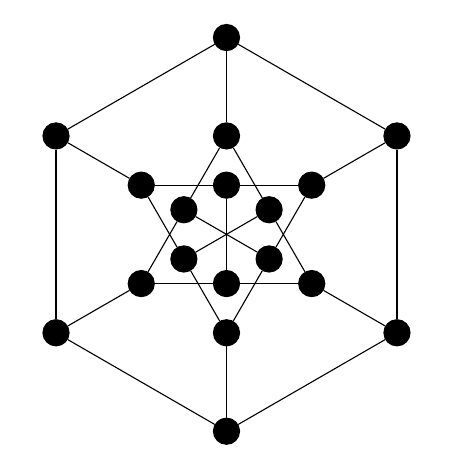
\begin{tikzpicture}[scale=0.5,
        vertex_style/.style={circle,draw=black,fill=black},edge_style/.style={draw=black}]

    \useasboundingbox (-5.05,-5.3) rectangle (5.1,5.25);

    \begin{scope}[rotate=90]
        \foreach \x/\y in {0/1,60/2,120/3,180/4,240/5,300/6}{
                \node[vertex_style] (\y) at (canvas polar cs: radius=2.5cm,angle=\x){};
            }
        \foreach \x/\y in {0/7,60/8,120/9,180/10,240/11,300/12}{
                \node[vertex_style] (\y) at (canvas polar cs: radius=5cm,angle=\x){};
            }

        \foreach \x/\y in {0/13,60/14,120/15,180/16,240/17,300/18}{
                \node[vertex_style] (\y) at (canvas polar cs: radius=1.25cm,angle=\x){};
            }

    \end{scope}

    \foreach \x/\y in {13/16,14/17,15/18}{
            \draw[edge_style] (\x) -- (\y);
        }

    \foreach \w/\x/\y/\z in {1/7/14/18,2/8/15/13,3/9/16/14,4/10/17/15,5/11/18/16,6/12/13/17}{
            \draw[edge_style] (\w) -- (\x);
            \draw[edge_style] (\w) -- (\y);
            \draw[edge_style] (\w) -- (\z);
        }

    \foreach \x/\y in {7/8,8/9,9/10,10/11,11/12,12/7}{
            \draw[edge_style] (\x) -- (\y);
        }
\end{tikzpicture}